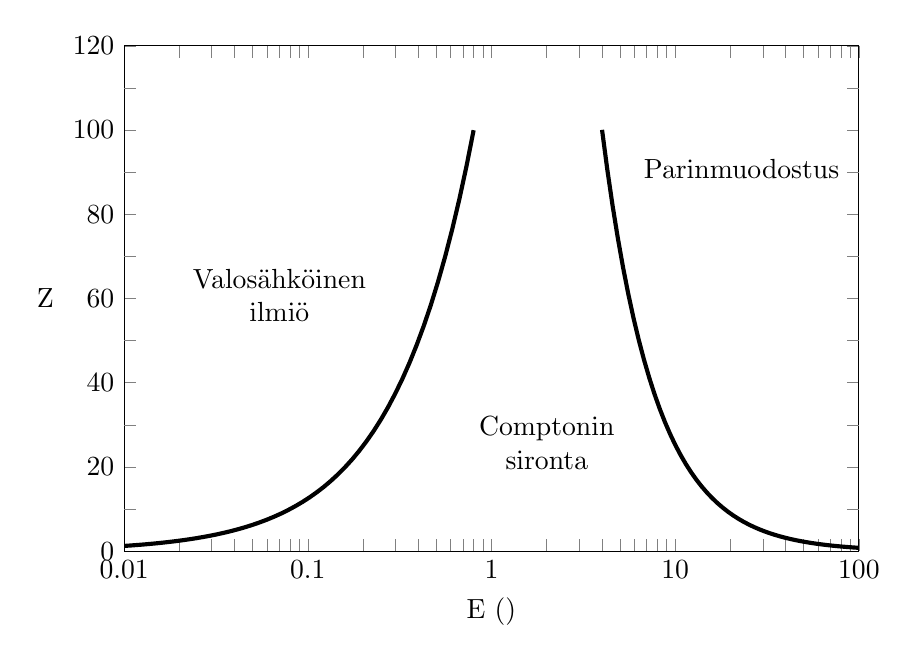
\begin{tikzpicture} %\cite{evans_atomic_1955}, sivu 712
    \begin{semilogxaxis}[
        width=.9\textwidth,
        height=8cm,
        xlabel={E (\unit{\mega\electronvolt})},
        ylabel={\rotatebox{-90}{Z}},
        xmin=0.01, xmax=100,
        ymin=0, ymax=120,
        xtick={0.01,0.1,1,10,100},
        ytick={0,20,40,60,80,100,120},
        grid=none,
        major grid style={line width=.2pt,draw=gray!50},
        minor tick style={draw=none},
        tick label style={
            /pgf/number format/fixed,
        },
        xticklabel={%
            \pgfkeys{/pgf/fpu=true}%
            \pgfmathparse{pow(10, \tick)}%
            \pgfmathprintnumber{\pgfmathresult}%
            \pgfkeys{/pgf/fpu=false}%
        },
        log basis x={10},
        extra x ticks={0.02, 0.03, 0.04, 0.05, 0.06, 0.07, 0.08, 0.09, 0.2, 0.3, 0.4, 0.5, 0.6, 0.7, 0.8, 0.9, 2, 3, 4, 5, 6, 7, 8, 9, 20, 30, 40, 50, 60, 70, 80, 90},
        extra x tick labels = {},
        extra y ticks={10,30,50,70,90,110},
        extra y tick labels = {},
        extra tick style={grid=none},
    ]
        \addplot[
            domain=0.01:0.8, 
            samples=50, 
            color=black,
            line width=1.5pt,
        ]
        {125*x};
        \addplot[
            domain=4:100, 
            samples=50, 
            color=black,
            line width=1.5pt,
        ]
        {800/x^(1.5)};
        \node at (axis cs:0.07,60) {\begin{tabular}{c} Valosähköinen \\ ilmiö \end{tabular}};
        \node at (axis cs:2,25) {\begin{tabular}{c} Comptonin \\ sironta \end{tabular}};
        \node at (axis cs:23,90) {\begin{tabular}{c} Parinmuodostus \end{tabular}};
    \end{semilogxaxis}
\end{tikzpicture}